\documentclass[tikz,border=4pt]{standalone}
\usepackage{tikz}
\usetikzlibrary{arrows.meta}

\begin{document}
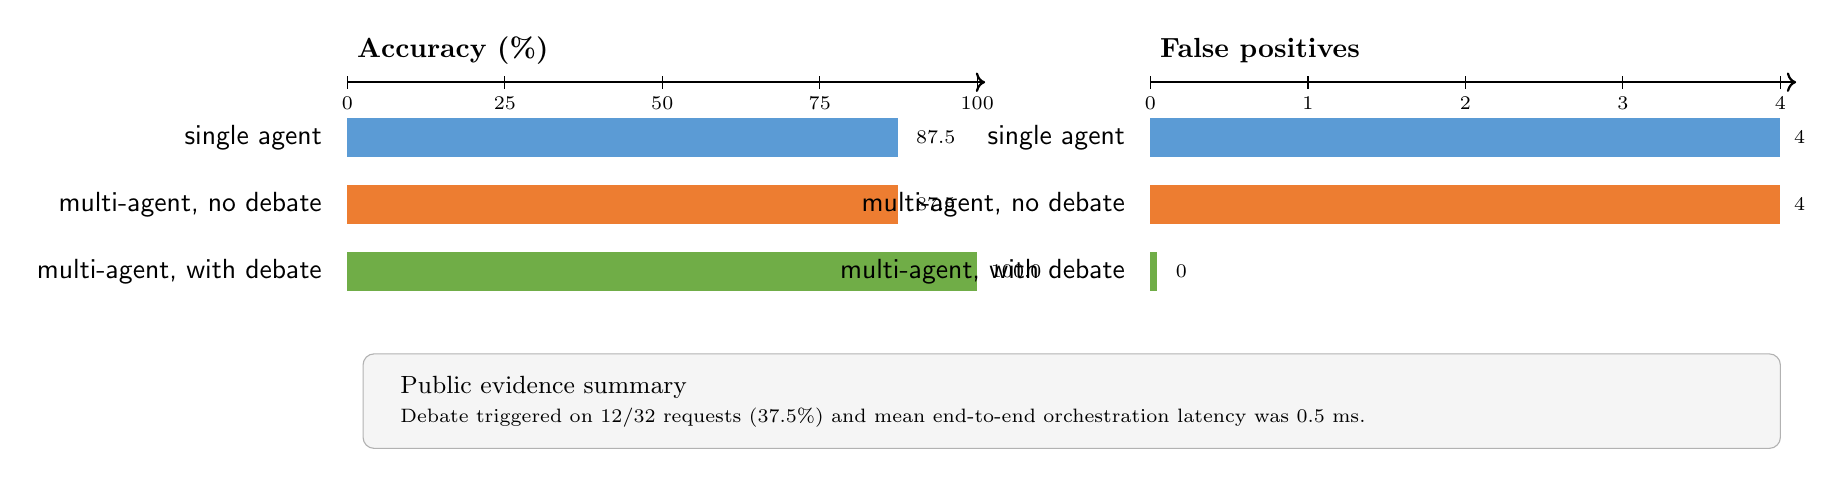
\begin{tikzpicture}[font=\sffamily]
  \definecolor{cOne}{RGB}{91,155,213}
  \definecolor{cTwo}{RGB}{237,125,49}
  \definecolor{cThree}{RGB}{112,173,71}

  \node[anchor=west, font=\bfseries] at (0,5.2) {Accuracy (\%)};
  \draw[->, thick] (0,4.8) -- (8.1,4.8);
  \foreach \x/\lab in {0/0,2/25,4/50,6/75,8/100}
    \draw (\x,4.72) -- (\x,4.88) node[below=4pt, font=\scriptsize] {\lab};
  \node[anchor=east] at (-0.2,4.1) {single agent};
  \node[anchor=east] at (-0.2,3.25) {multi-agent, no debate};
  \node[anchor=east] at (-0.2,2.4) {multi-agent, with debate};
  \fill[cOne] (0,3.85) rectangle (7.0,4.35);
  \fill[cTwo] (0,3.0) rectangle (7.0,3.5);
  \fill[cThree] (0,2.15) rectangle (8.0,2.65);
  \node[anchor=west, font=\scriptsize] at (7.1,4.1) {87.5};
  \node[anchor=west, font=\scriptsize] at (7.1,3.25) {87.5};
  \node[anchor=west, font=\scriptsize] at (8.05,2.4) {100.0};

  \node[anchor=west, font=\bfseries] at (10.2,5.2) {False positives};
  \draw[->, thick] (10.2,4.8) -- (18.4,4.8);
  \foreach \x/\lab in {10.2/0,12.2/1,14.2/2,16.2/3,18.2/4}
    \draw (\x,4.72) -- (\x,4.88) node[below=4pt, font=\scriptsize] {\lab};
  \node[anchor=east] at (10.0,4.1) {single agent};
  \node[anchor=east] at (10.0,3.25) {multi-agent, no debate};
  \node[anchor=east] at (10.0,2.4) {multi-agent, with debate};
  \fill[cOne] (10.2,3.85) rectangle (18.2,4.35);
  \fill[cTwo] (10.2,3.0) rectangle (18.2,3.5);
  \fill[cThree] (10.2,2.15) rectangle (10.28,2.65);
  \node[anchor=west, font=\scriptsize] at (18.25,4.1) {4};
  \node[anchor=west, font=\scriptsize] at (18.25,3.25) {4};
  \node[anchor=west, font=\scriptsize] at (10.4,2.4) {0};

  \draw[rounded corners=4pt, fill=gray!8, draw=gray!60] (0.2,0.15) rectangle (18.2,1.35);
  \node[anchor=west, font=\small] at (0.55,0.92) {Public evidence summary};
  \node[anchor=west, font=\scriptsize] at (0.55,0.54) {Debate triggered on 12/32 requests (37.5\%) and mean end-to-end orchestration latency was 0.5 ms.};
\end{tikzpicture}
\end{document}
